\documentclass[12pt,a4paper]{article}
 
\usepackage{float}
%für feststellen der figures und tables [H] dranschreiben
\usepackage{units}
%wird so benutzt: 
%\unit[value/Zahl]{dimension/Einheit} oder 
%\unitfrac[value/Zahl]{dimension/Einheit num/Zähler}{dimension/Einheit denum/Nenner} oder
%\nicefrac[fontcommand/Schriftart]{dimension/Einheit num/Zähler}{dimension/Einheit denum/Nenner}

\usepackage{caption}
\usepackage{subcaption}

\usepackage[left=2cm,right=2cm,top=2cm,bottom=2cm]{geometry}
\usepackage[utf8]{inputenc}
\usepackage[T1]{fontenc}
\usepackage{lmodern}
\usepackage[ngerman]{babel}
\usepackage{amsmath}
\usepackage{graphicx}
 
\title{Der Transistor}
\author{Frederik Strothmann, Henrik Jürgens}
\date{\today}
%niemals zwei überschriften direkt übereinander schreiben, also immer mindestens in einem satz was sinnvolles unter jede überschrift schreiben (bei den versuchen z.B. das versuchsziel) 
\begin{document}
%deckblatt erstellen.
\maketitle
\newpage
\tableofcontents
\newpage
\section{Einleitung}
%einleitung zu dem experiment.
%auf die einstellungen, die vor dem versuch gemacht werden, eingehen oder auf eine anleitung dazu verweisen
%es soll immer erwähnt werden um was es in dem Versuch geht und wie das relisiert werden soll
Dieser Versuch beschäftigt sich mit Transistoren, dem zentralen Verstärkerelement der Halbleitertechnik. Die elektrischen Eigenschaften dieses Schaltelements sollen über die Aufnahme von Kennlinien untersucht werden. Danach werden Schaltungen aufgebaut, welche Ströme oder Spannungen verstärken sollen. Während des Versuches sollen die Eigenschaften des Bipolartransistors (NPN oder PNP) sowie des Feldeffekttransistor (FET) kennengelernt werden, sowie Schaltungen zur Wechselspannungsverstärkung und Gleichspannungstabilisierung aufgebaut werden. Falls noch Zeit ist, können Signale von Sensoren mithilfe von Transistoren weiterverarbeitet werden.\footnote{vgl. Zielsetzung des Versuches http://www.atlas.uni-wuppertal.de/$\sim$kind/ep3\_14.pdf am 09.11.2014}
%---------------------------------------------------------------------------------------------
%hinter der einleitung kann der allgemeine theoretische hintergrund in einer zusätzlichen section erklärt werden
%1-----------------------------------------------1
\section{Eigenschaften von Transistoren}
%kurz das ziel dieses versuchsteiles ansprechen, damit keine zwei überschriften direkt übereinander stehen!
%bei schwierigeren versuchen kann auch der theoretische hintergrund erläutert werden. (mit formeln, herleitungen und erklärungen)
Ziel dieses Versuchsteils ist es die Ausgangs und Eingangskennlinie eines Transistors aufzunehmen, sowie die Stromverstärkung zu bestimmen.
\subsection{Verwendete Geräte}
%(immer) eine skizze oder ein foto einfügen, die geräte/materialien !nummerieren! und z.b. eine legende dazu schreiben, besser wäre es das ganze in einem Fließtext gut zu beschreiben.
%falls am anfang des versuches nicht klar ist, was alles verwendet wird, wenn möglich erst am ende ein großes foto von den verwendeten materialien machen!\\
\subsection{Verwendete Formeln}
%eine legende kann angefertigt werden, die selbstverständlichen buchstaben müssen nicht extra erklärt werden
%mit knappen erklärungen die !verwendeten! formeln, sowie die zugehörige fehlerrechnung einfügen
%2-----------------------------------------------2
%ab hier kann nochmal in einzelne versuchsteile unterteilt werden
\subsection{Versuchsaufbau}
%skizze zum versuchsaufbau (oder foto) einfügen,   es muss erklärt werden wie das ganze funktioniert und welche speziellen einstellungen verwendet wurden (z.b. welche knöpfe an den geräten für die messung verdreht wurden)

\begin{itemize}
\item	T1 BC550

\item	R$_1$ 10k$\Omega$

\item	U$_2$ 5V (Eingangslinie)

\item	U$_2$ 0-10V (Ausgangslinie)
\end{itemize}

\begin{figure}[H] 
  \centering
    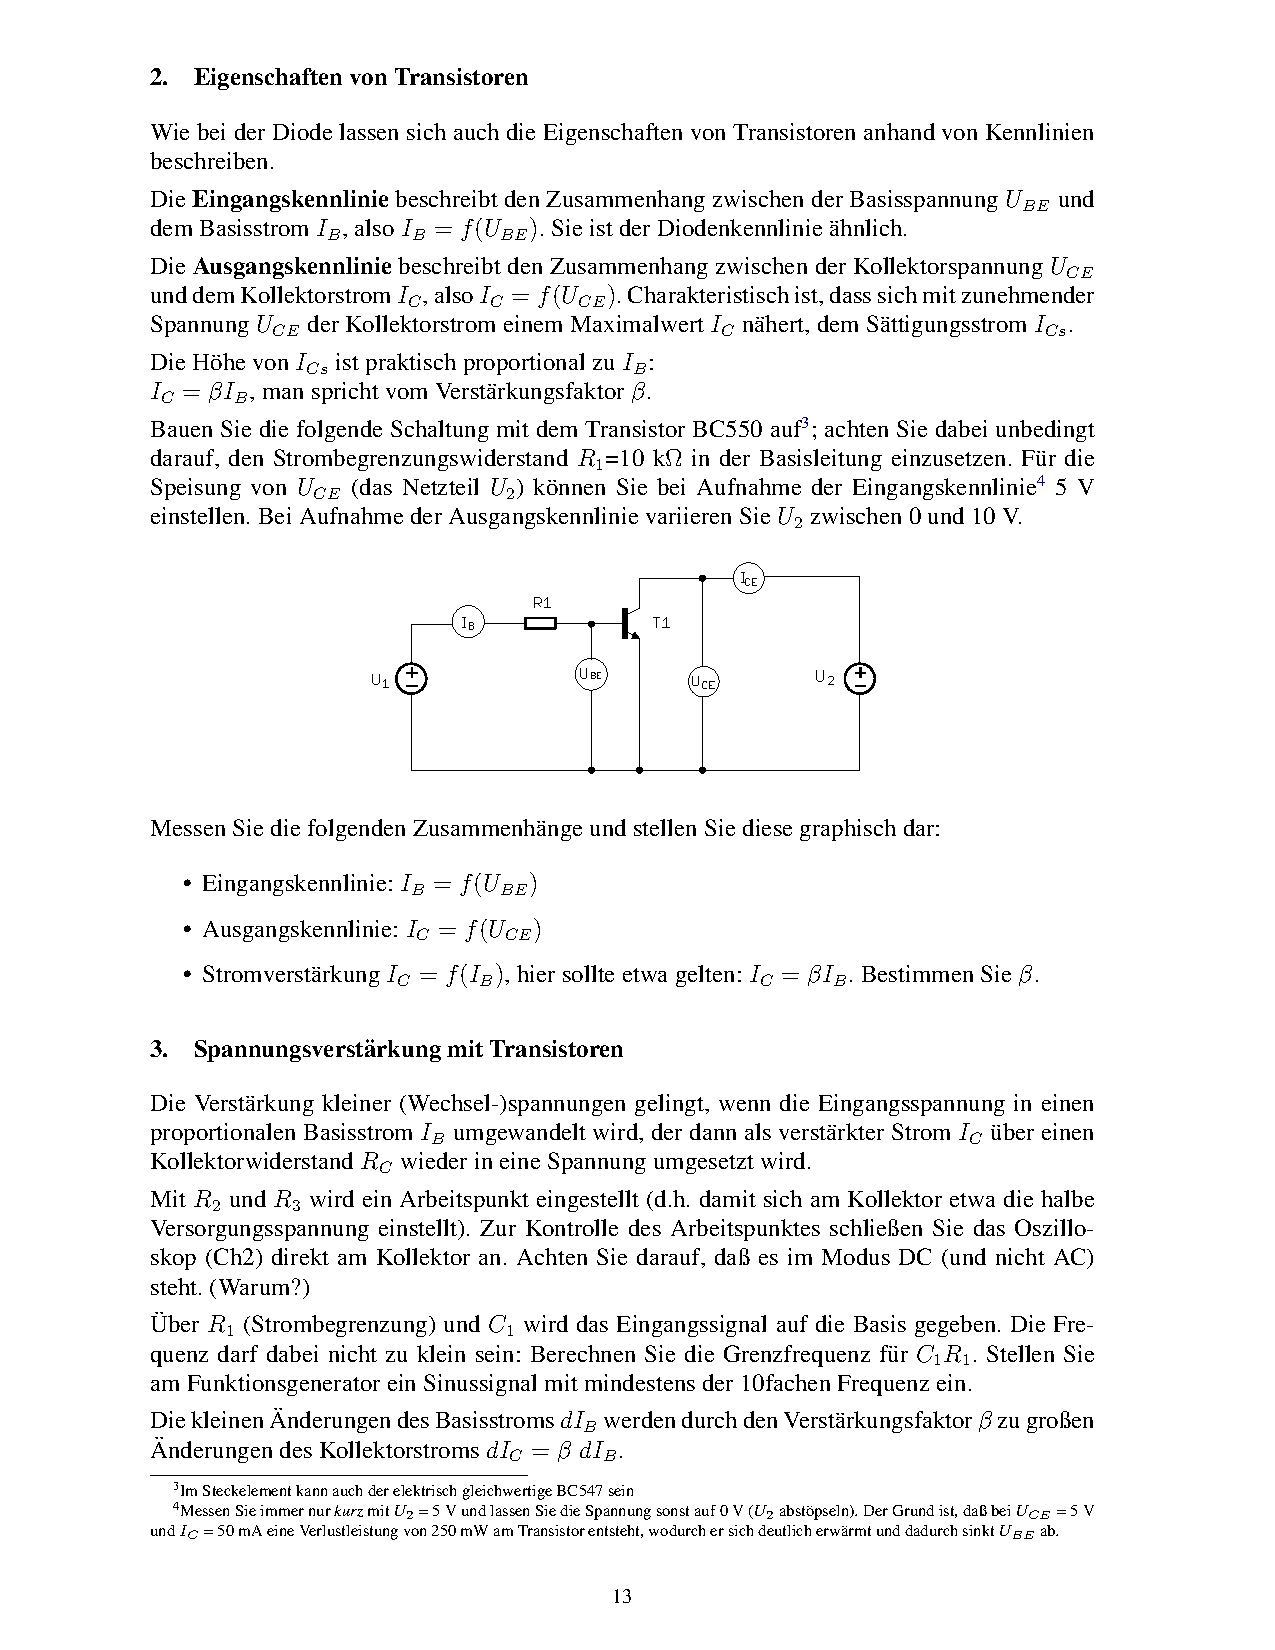
\includegraphics[trim = 10mm 145mm 10mm 90mm, clip, scale = 1]{ep3_14[Page13].pdf}
  	\caption[Schaltskizze für die Messung der Ein- und Ausgangskennlinie eines Transistors]{Schaltskizze für die Messung der Ein- und Ausgangskennlinie eines Transistors\footnotemark}
  \label{fig:1}
\end{figure}
\footnotetext{Abbildung entnommen von http://www.atlas.uni-wuppertal.de/$\sim$kind/ep3\_14.pdf Seite 13 am 10.11.2014}

\subsection{Versuchsdurchführung}
%erklären, !was! wir machen, !warum! wir das machen und mit welchem ziel
%(wichtig) präzize erklären, wie bei dem versuch vorgegangen und was gemacht wurde
Zuerst soll die Eingangskennlinie  $I_B$ gegen $U_{BE}$ aufgenommen werden. Zu erwarten ist ein diodenähnlicher exponentieller Zusammenhang, wobei die Spannung $U_{CE}$  bei dieser Messung auf \unit[5]{V} gestellt wird ($I_B = f(U_{BE})$). Danach wird die Ausgangskennlinie $I_C$ gegen $U_{CE}$ aufgenommen.
Anschließend soll die Stromverstärkung $\beta$ zwischen $I_B$ und $I_C$ bestimmt werden ($I_C = f(I_B)$). Es muss dabei beachtet werden, dass die Spannung $U_{BE}$ kleiner als die Spannung $U_{CE}$ bleibt, da $I_C$ nur für relativ kleine Ströme $I_B$ linear von $I_B$ abhängt.
\subsection{Messergebnisse}
%die messwerte in !übersichtlichen! tabellen angegeben
%zu viele kleine tabellen in große tabellen überführen!
%zu große tabellen mit dem [scale]-befehl scalieren oder (falls zu lang) in zwei kleinere tabellen aufteilen
%(wichtig) vor !jeder! tabelle sagen, was gemessen wurde und wie die fehler gewählt wurden und ausreichend !erklären!, !warum! wir unsere fehler grade so gewählt haben
\subsection{Auswertung}
%zuerst !alle! errechneten werte entweder in ganzen sätzen aufzählen, oder in tabellen (übersichtlicher) dargestellen, sowie auf die verwendeten formeln verweisen (die referenzierung der formel kann in der überschrift stehen)
%kurz erwähnen (vor der tabelle), warum wir das ganze ausrechnen bzw. was wir dort ausrechnen
%danach histogramme und plots erstellen, wobei wenn möglich funktionen durch die plots gelegt werden (zur not können auch splines benutzt werden, was aber angegeben werden muss)
%bei fits immer die funktion und das reduzierte chiquadrat mit angegeben, wobei auf verständlichkeit beim entziffern der zehnerpotenzen geachtet werden muss z.b. f(x)=(wert+-fehler)\cdot10^{irgendeine zahl}\cdot x + (wert+-fehler)\cdot10^{irgendeine zahl}
%bei jedem fit erklären, nach welchem zusammenhang gefittet wurde und warum!
%bei plots darauf achten, dass die achsenbeschriftung (auch die tics) die richtige größe haben und die legende im plot nicht die messwerte verdeckt
%kurz die aufgabenstellung abgehandeln
%2-----------------------------------------------2
\subsection{Diskussion}
%(immer) die gemessenen werte und die bestimmten werte über die messfehler mit literaturwerten oder untereinander vergleichen
%in welchem fehlerintervall des messwertes liegt der literaturwert oder der vergleichswert?
%wie ist der relative anteil des fehlers am messwert und damit die qualität unserer messung?
%in einem satz erklären, wie gut unser fehler und damit unsere messung ist
%kurz erläutern, wie systematische fehler unsere messung beeinflusst haben könnten
%(wichtig) zum schluss ansprechen, in wie weit die ergebnisse mit der theoretischen vorhersage übereinstimmen
%--------------------------------------------------------------------------------------------
%falls tabellen mit den messwerten zu lang werden, kann die section mit den messwerten auch hinter der diskussion angefügt bzw. eine section mit dem anhang eingefügt werden.
%1-----------------------------------------------1
\section{Spannungsverstärkung mit Transistoren}
%kurz das ziel dieses versuchsteiles ansprechen, damit keine zwei überschriften direkt übereinander stehen!
%bei schwierigeren versuchen kann auch der theoretische hintergrund erläutert werden. (mit formeln, herleitungen und erklärungen)
Ziel dieses Versuches ist die Verstärkung kleiner Wechselspannungen mithilfe des Transistors.
\subsection{Verwendete Geräte}
%(immer) eine skizze oder ein foto einfügen, die geräte/materialien !nummerieren! und z.b. eine legende dazu schreiben, besser wäre es das ganze in einem Fließtext gut zu beschreiben.
%falls am anfang des versuches nicht klar ist, was alles verwendet wird, wenn möglich erst am ende ein großes foto von den verwendeten materialien machen!\\
\subsection{Verwendete Formeln}
%eine legende kann angefertigt werden, die selbstverständlichen buchstaben müssen nicht extra erklärt werden
%mit knappen erklärungen die !verwendeten! formeln, sowie die zugehörige fehlerrechnung einfügen
%2-----------------------------------------------2
%ab hier kann nochmal in einzelne versuchsteile unterteilt werden
\subsection{Versuchsaufbau}
%skizze zum versuchsaufbau (oder foto) einfügen,   es muss erklärt werden wie das ganze funktioniert und welche speziellen einstellungen verwendet wurden (z.b. welche knöpfe an den geräten für die messung verdreht wurden)

\begin{itemize}
\item	T1 BC550

\item	C1 100nF

\item	R1 1k$\Omega$

\item	R2 100k$\Omega$

\item	R3 10k$\Omega$

\item	R4 1k$\Omega$ oder 10k$\Omega$

\item	C2 1$\mu$F

\item	Versorgungsspannung 10V
\end{itemize}

\begin{figure}[H] 
  \centering
    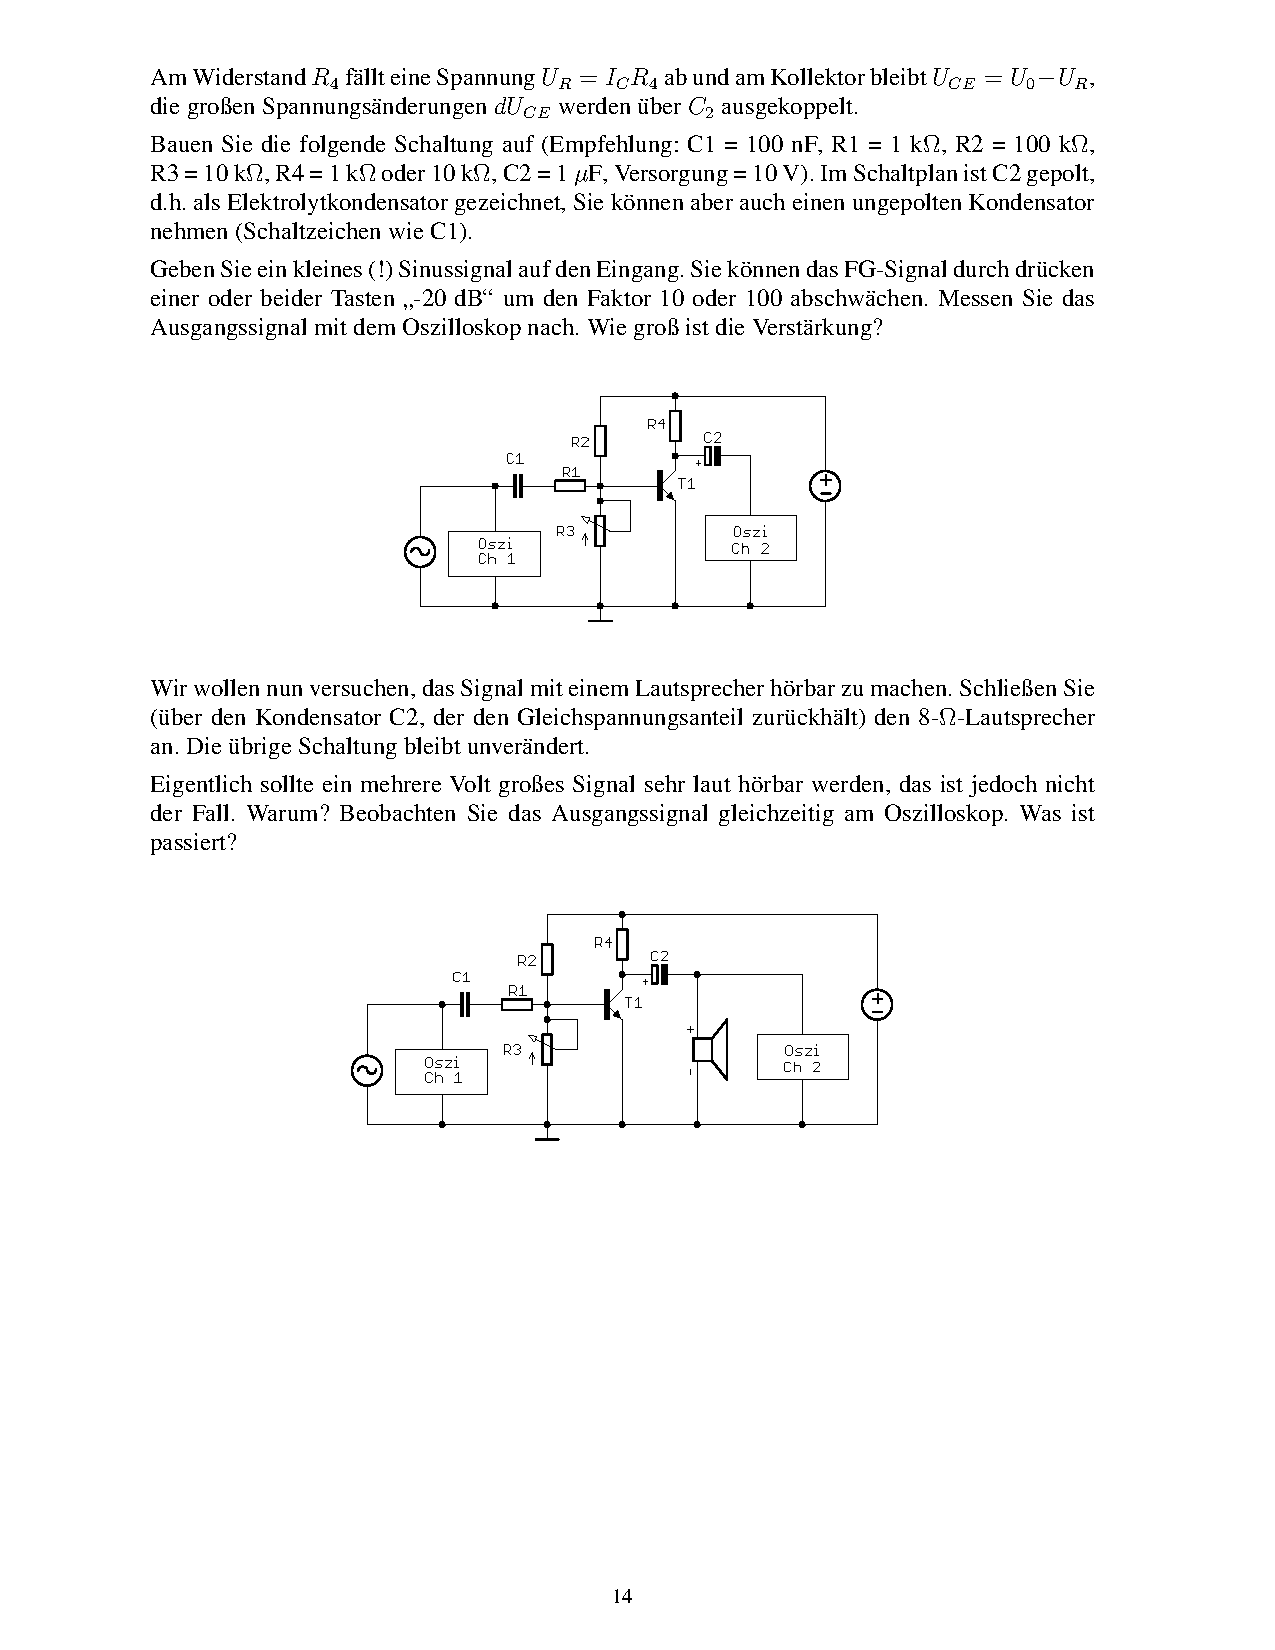
\includegraphics[trim = 10mm 165mm 10mm 60mm, clip, scale = 1]{ep3_14[Page14].pdf}
  	\caption[Schaltskizze für die Messung des Spannungsverstärkungsfaktors]{Schaltskizze für die Messung des Spannungsverstärkungsfaktors\footnotemark}
  \label{fig:2}
\end{figure}
\footnotetext{Abbildung entnommen von http://www.atlas.uni-wuppertal.de/$\sim$kind/ep3\_14.pdf Seite 14 am 10.11.2014}


\begin{itemize}
\item	T1 BC550

\item	C1 100nF

\item	R1 1k$\Omega$

\item	R2 100k$\Omega$

\item	R3 10k$\Omega$

\item	R4 1k$\Omega$ oder 10k$\Omega$

\item	C2 1$\mu$F

\item	Versorgungsspannung 10V

\item	8$\Omega$ Lautsprecher
\end{itemize}

\begin{figure}[H] 
  \centering
    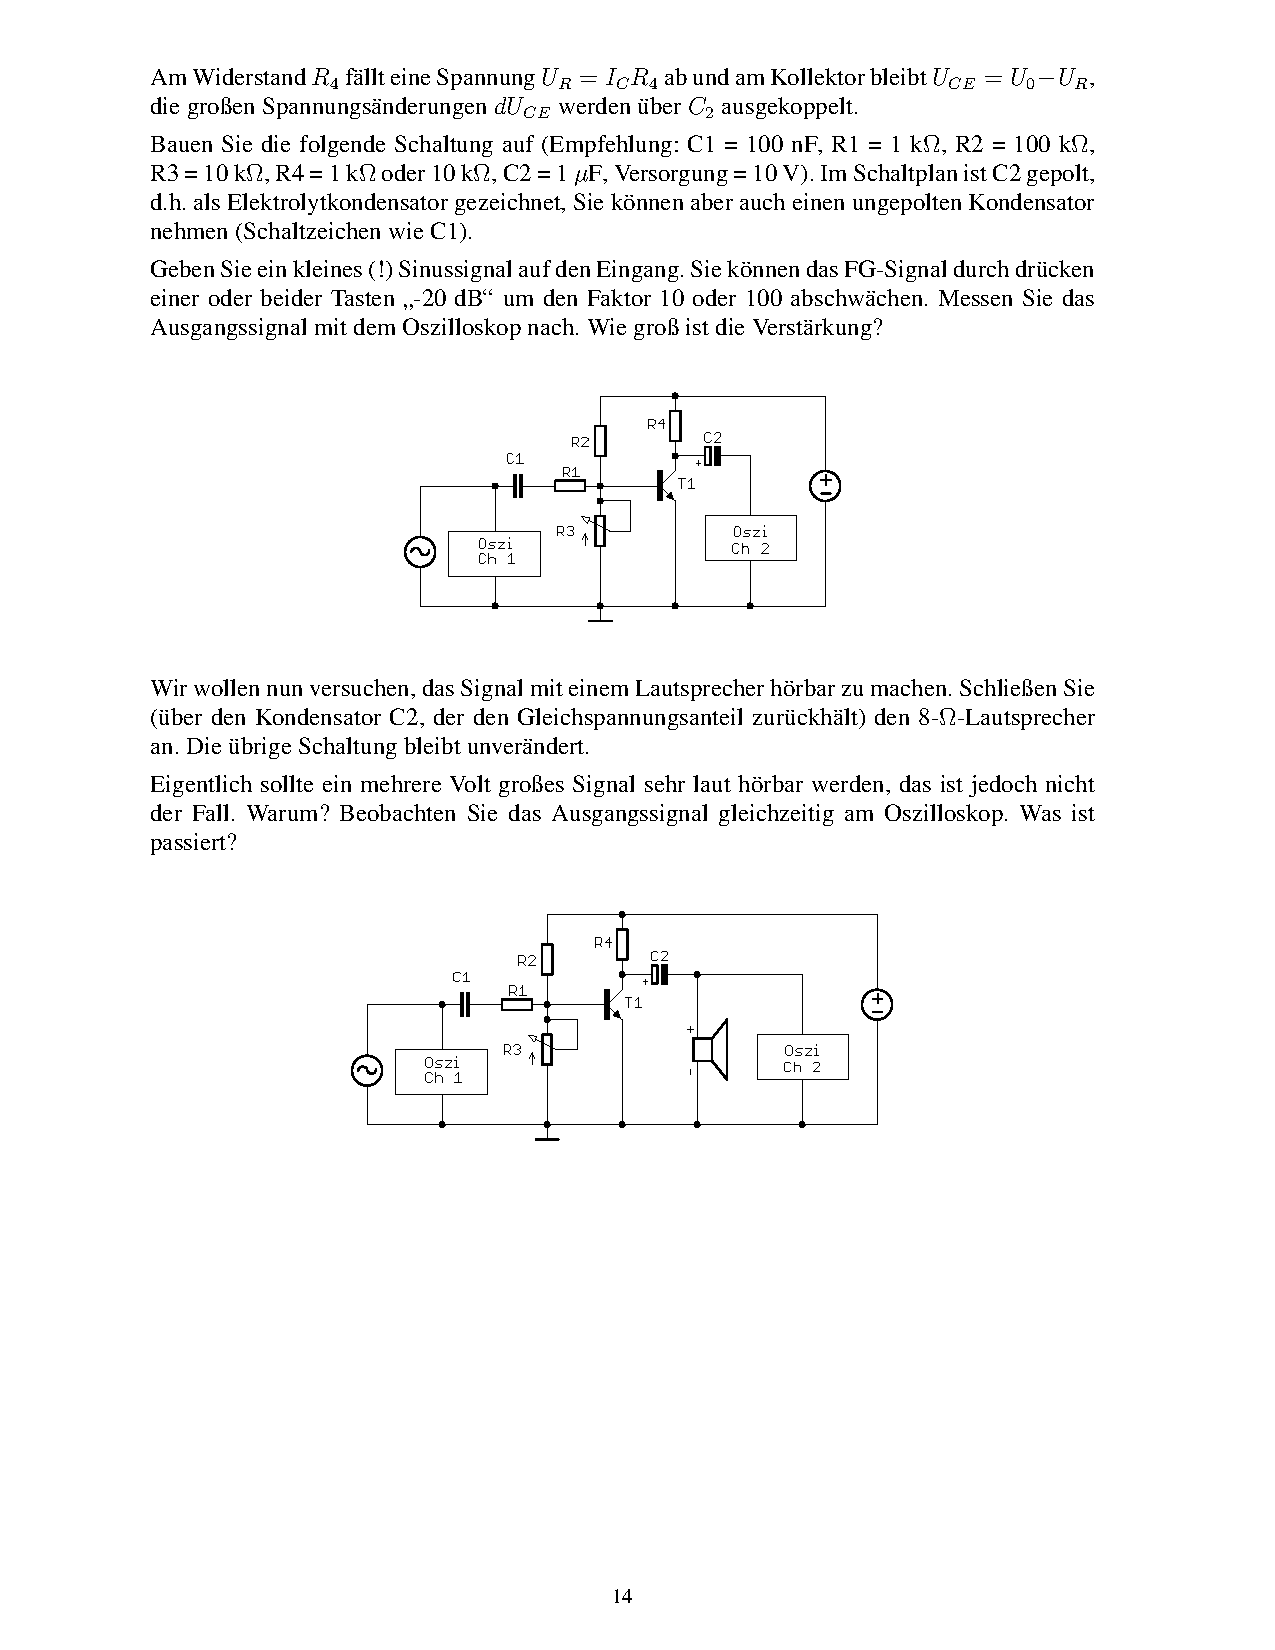
\includegraphics[trim = 10mm 65mm 10mm 150mm, clip, scale = 1]{ep3_14[Page14].pdf}
  	\caption[Schaltskizze für die Messung des Spannungsverstärkungsfaktors und Audioausgabe des verstärkten Signals]{Schaltskizze für die Messung des Spannungsverstärkungsfaktors und Audioausgabe des verstärkten Signals\footnotemark}
  \label{fig:3}
\end{figure}
\footnotetext{Abbildung entnommen von http://www.atlas.uni-wuppertal.de/$\sim$kind/ep3\_14.pdf Seite 14 am 10.11.2014}

\subsection{Versuchsdurchführung}
%erklären, !was! wir machen, !warum! wir das machen und mit welchem ziel
%(wichtig) präzize erklären, wie bei dem versuch vorgegangen und was gemacht wurde
Mit dem Oszilloskop werden Ausgangs- und Eingangssignal bei der Schaltung für die Spannungsverstärkung aufgenommen, um den Verstärkungsfaktor zwischen Ausgangs und Eingangsspannung zu bestimmen. Im zweiten Teil soll ein Lautsprecher über den Kondensator angeschlossen werden. Da der Strom nur auf wenige Milliampere beschränkt ist, ist zu erwarten, dass die Spannung an dem niederohmigen Lautsprecher zusammenbricht und damit kaum etwas zu hören ist.
\subsection{Messergebnisse}
%die messwerte in !übersichtlichen! tabellen angegeben
%zu viele kleine tabellen in große tabellen überführen!
%zu große tabellen mit dem [scale]-befehl scalieren oder (falls zu lang) in zwei kleinere tabellen aufteilen
%(wichtig) vor !jeder! tabelle sagen, was gemessen wurde und wie die fehler gewählt wurden und ausreichend !erklären!, !warum! wir unsere fehler grade so gewählt haben
\subsection{Auswertung}
%zuerst !alle! errechneten werte entweder in ganzen sätzen aufzählen, oder in tabellen (übersichtlicher) dargestellen, sowie auf die verwendeten formeln verweisen (die referenzierung der formel kann in der überschrift stehen)
%kurz erwähnen (vor der tabelle), warum wir das ganze ausrechnen bzw. was wir dort ausrechnen
%danach histogramme und plots erstellen, wobei wenn möglich funktionen durch die plots gelegt werden (zur not können auch splines benutzt werden, was aber angegeben werden muss)
%bei fits immer die funktion und das reduzierte chiquadrat mit angegeben, wobei auf verständlichkeit beim entziffern der zehnerpotenzen geachtet werden muss z.b. f(x)=(wert+-fehler)\cdot10^{irgendeine zahl}\cdot x + (wert+-fehler)\cdot10^{irgendeine zahl}
%bei jedem fit erklären, nach welchem zusammenhang gefittet wurde und warum!
%bei plots darauf achten, dass die achsenbeschriftung (auch die tics) die richtige größe haben und die legende im plot nicht die messwerte verdeckt
%kurz die aufgabenstellung abgehandeln
%2-----------------------------------------------2
\subsection{Diskussion}
%(immer) die gemessenen werte und die bestimmten werte über die messfehler mit literaturwerten oder untereinander vergleichen
%in welchem fehlerintervall des messwertes liegt der literaturwert oder der vergleichswert?
%wie ist der relative anteil des fehlers am messwert und damit die qualität unserer messung?
%in einem satz erklären, wie gut unser fehler und damit unsere messung ist
%kurz erläutern, wie systematische fehler unsere messung beeinflusst haben könnten
%(wichtig) zum schluss ansprechen, in wie weit die ergebnisse mit der theoretischen vorhersage übereinstimmen
%--------------------------------------------------------------------------------------------
%falls tabellen mit den messwerten zu lang werden, kann die section mit den messwerten auch hinter der diskussion angefügt bzw. eine section mit dem anhang eingefügt werden.
%1-----------------------------------------------1
\section{Stromverstärkung mit Transistoren}
%kurz das ziel dieses versuchsteiles ansprechen, damit keine zwei überschriften direkt übereinander stehen!
%bei schwierigeren versuchen kann auch der theoretische hintergrund erläutert werden. (mit formeln, herleitungen und erklärungen)
Neben der Spannungsverstärkung kann mit dem Transistor auch der Strom verstärkt werden, um höhere Ausgangsströme zu erreichen.
\subsection{Verwendete Geräte}
%(immer) eine skizze oder ein foto einfügen, die geräte/materialien !nummerieren! und z.b. eine legende dazu schreiben, besser wäre es das ganze in einem Fließtext gut zu beschreiben.
%falls am anfang des versuches nicht klar ist, was alles verwendet wird, wenn möglich erst am ende ein großes foto von den verwendeten materialien machen!\\
\subsection{Verwendete Formeln}
%eine legende kann angefertigt werden, die selbstverständlichen buchstaben müssen nicht extra erklärt werden
%mit knappen erklärungen die !verwendeten! formeln, sowie die zugehörige fehlerrechnung einfügen
%2-----------------------------------------------2
%ab hier kann nochmal in einzelne versuchsteile unterteilt werden
\subsection{Versuchsaufbau}
%skizze zum versuchsaufbau (oder foto) einfügen,   es muss erklärt werden wie das ganze funktioniert und welche speziellen einstellungen verwendet wurden (z.b. welche knöpfe an den geräten für die messung verdreht wurden)

\begin{itemize}
\item	T1 BD137

\item	R1 10k$\Omega$

\item	R2 1k$\Omega$

\item	R3 100$\Omega$

\item	Versorgungsspannung 10V

\end{itemize}

\begin{figure}[H] 
  \centering
    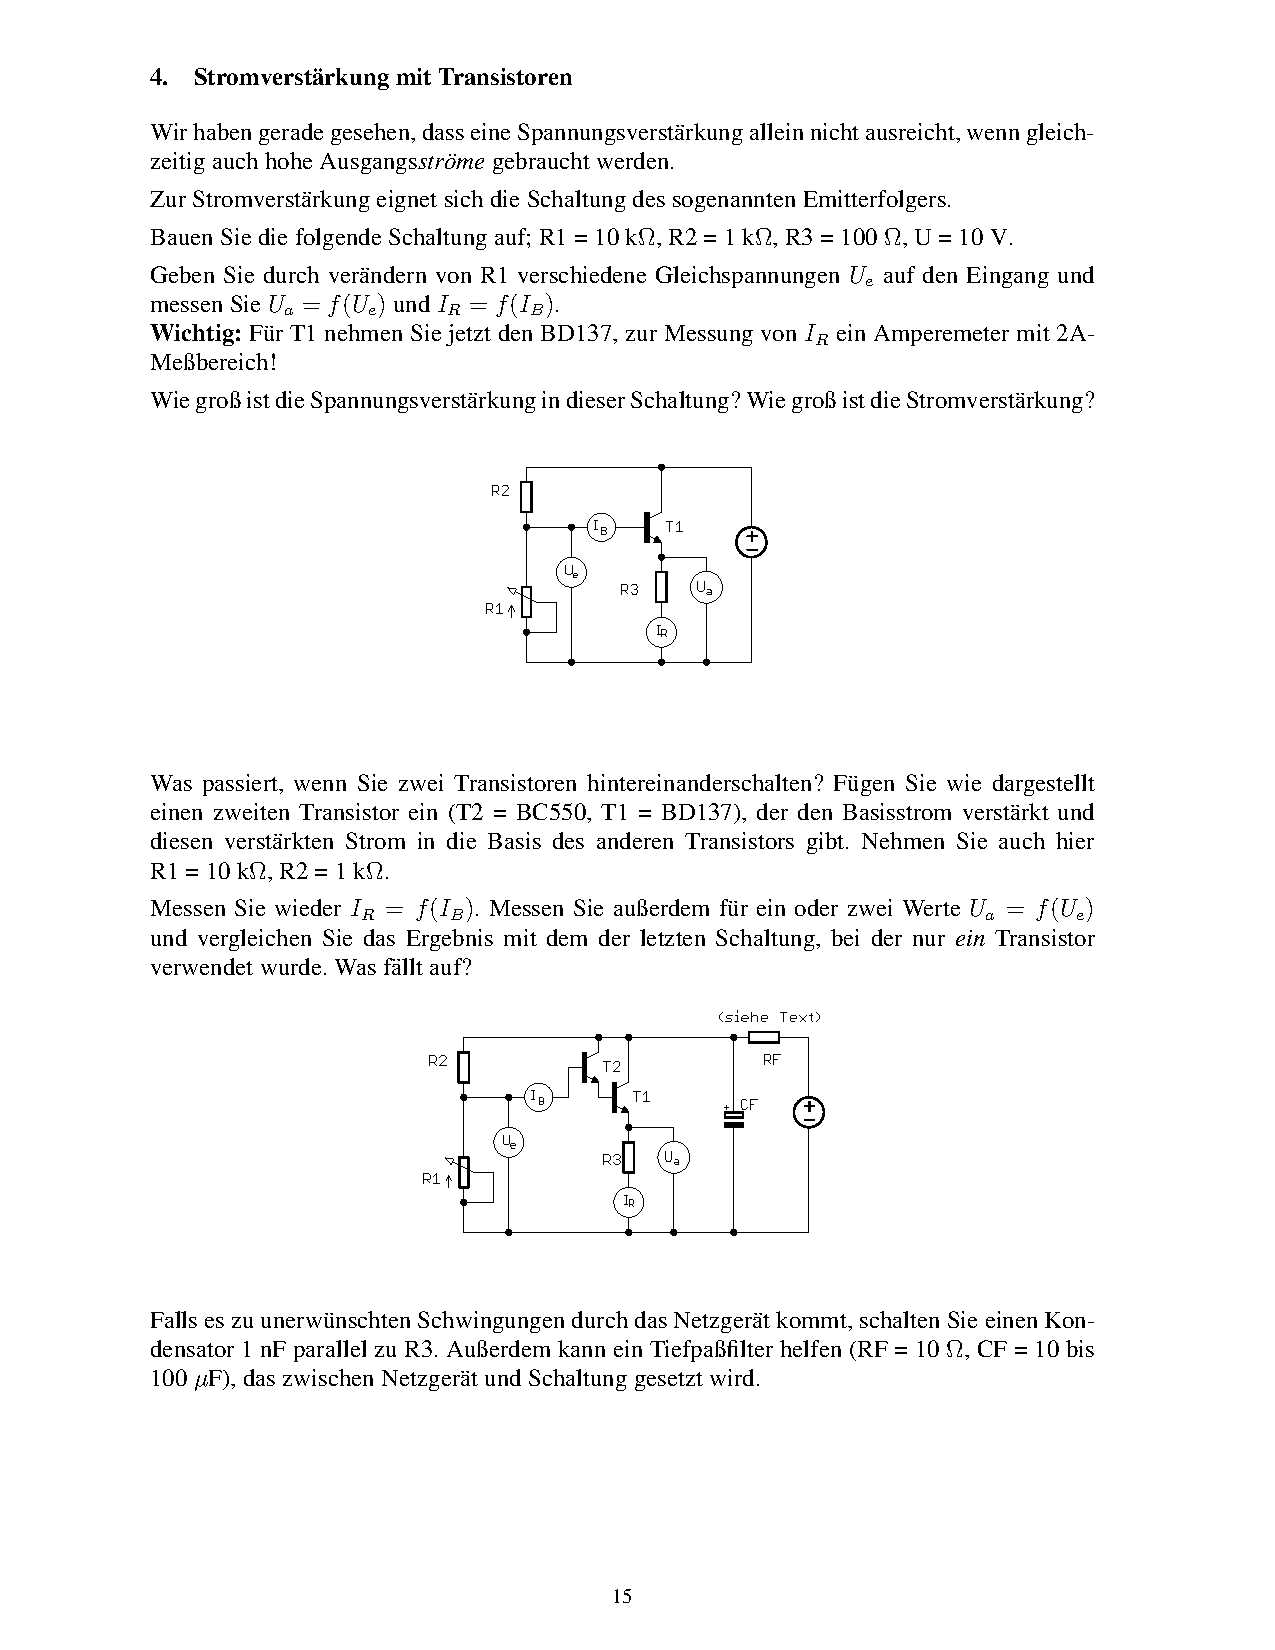
\includegraphics[trim = 10mm 165mm 10mm 75mm, clip, scale = 1]{ep3_14[Page15].pdf}
  	\caption[Schaltskizze für die Messung des Stromverstärkungsfaktors]{Schaltskizze für die Messung des Stromverstärkungsfaktors\footnotemark}
  \label{fig:4}
\end{figure}
\footnotetext{Abbildung entnommen von http://www.atlas.uni-wuppertal.de/$\sim$kind/ep3\_14.pdf Seite 15 am 10.11.2014}


\begin{itemize}
\item	T1 BD137

\item	T2 BC550

\item	R1 10k$\Omega$

\item	R2 1k$\Omega$

\item	R3 100$\Omega$

\item	Versorgungsspannung 10V

\item	CF 10-100$\mu$F

\end{itemize}

\begin{figure}[H] 
  \centering
    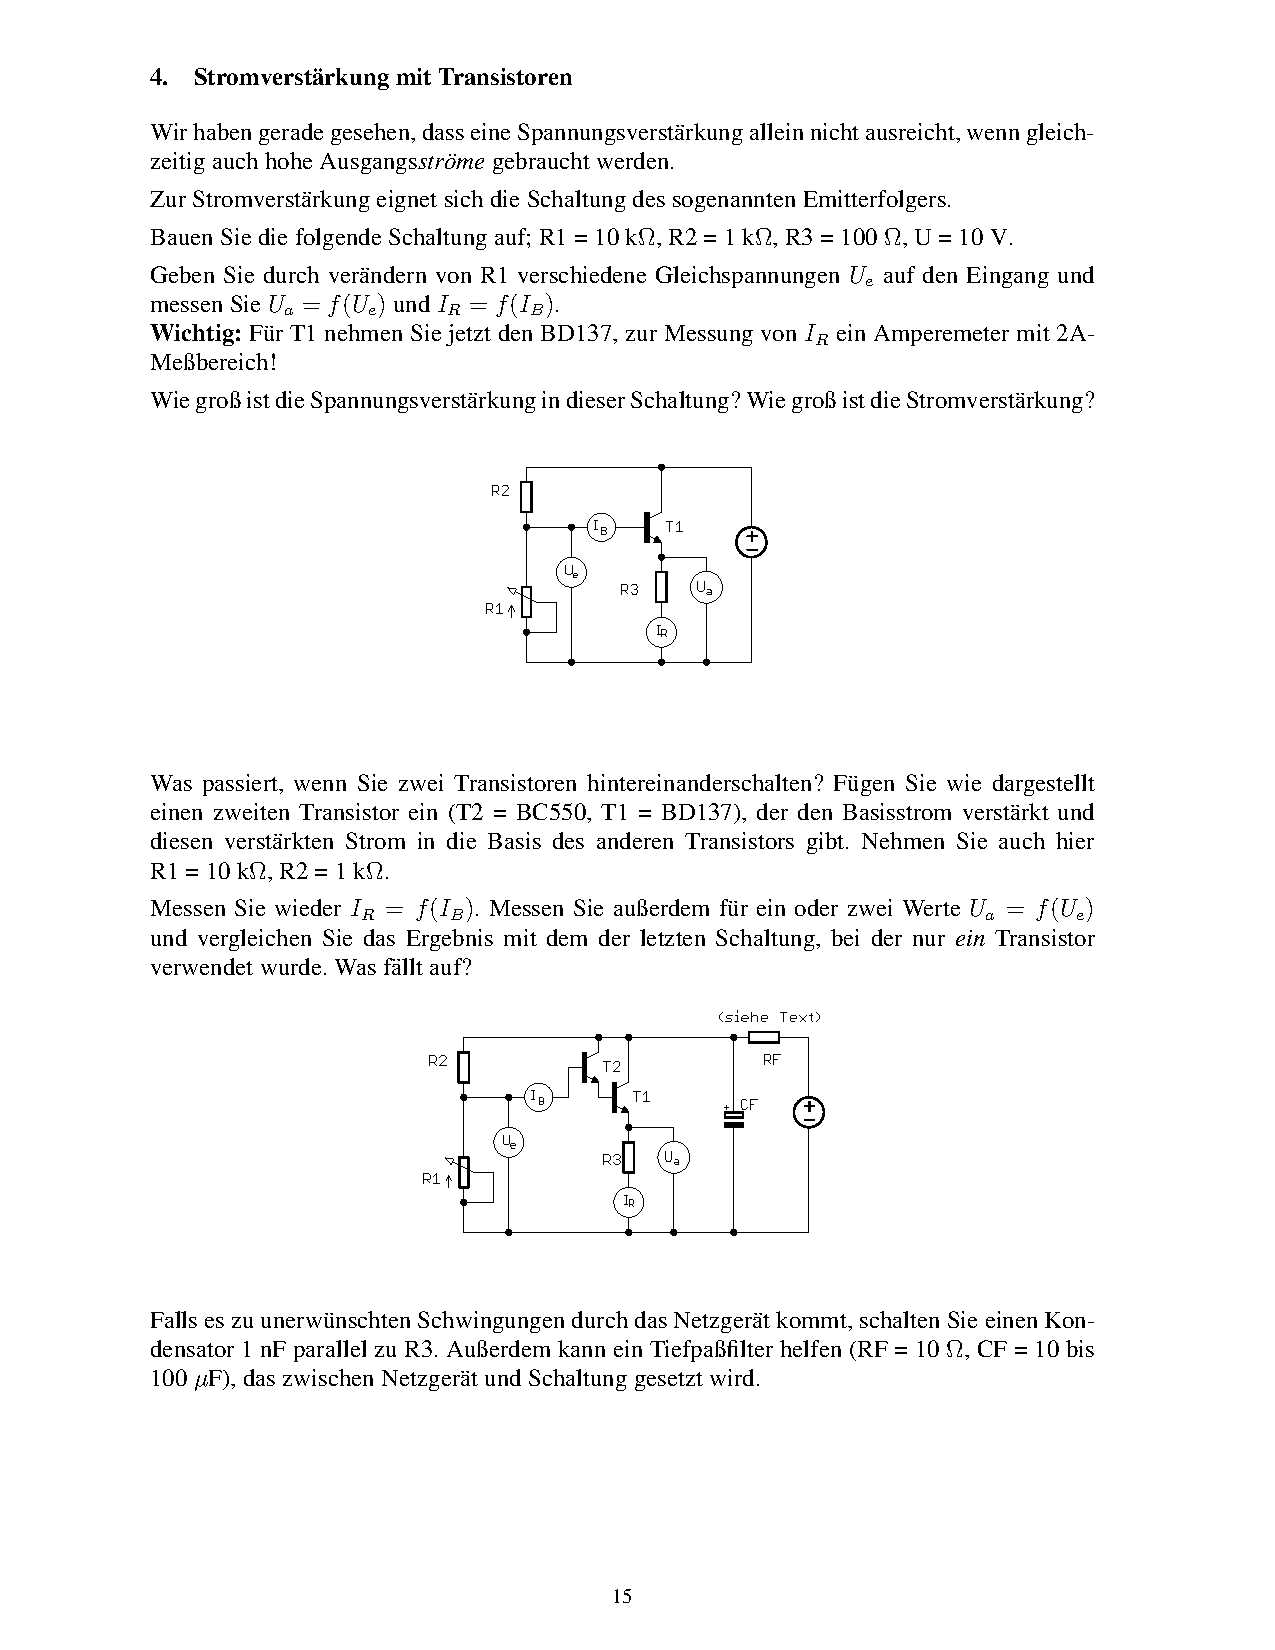
\includegraphics[trim = 10mm 65mm 10mm 174mm, clip, scale = 1]{ep3_14[Page15].pdf}
  	\caption[Schaltskizze für die Messung des Stromverstärkungsfaktors mit zwei hinter einander geschalteten Transistoren]{Schaltskizze für die Messung des Stromverstärkungsfaktors mit zwei hinter einander geschalteten Transistoren\footnotemark}
  \label{fig:5}
\end{figure}
\footnotetext{Abbildung entnommen von http://www.atlas.uni-wuppertal.de/$\sim$kind/ep3\_14.pdf Seite 15 am 10.11.2014}

\begin{itemize}
\item	T1 BD137

\item	T2 BC550

\item	C1 1$\mu$F

\item	R1 1k$\Omega$

\item	R2 100k$\Omega$

\item	R3 10k$\Omega$

\item	R4 1k$\Omega$

\item	R5 100$\Omega$

\item	R4 1k$\Omega$ oder 10k$\Omega$

\item	C2 100$\mu$F

\item	CF 10-100$\mu$F
\end{itemize}

\begin{figure}[H] 
  \centering
    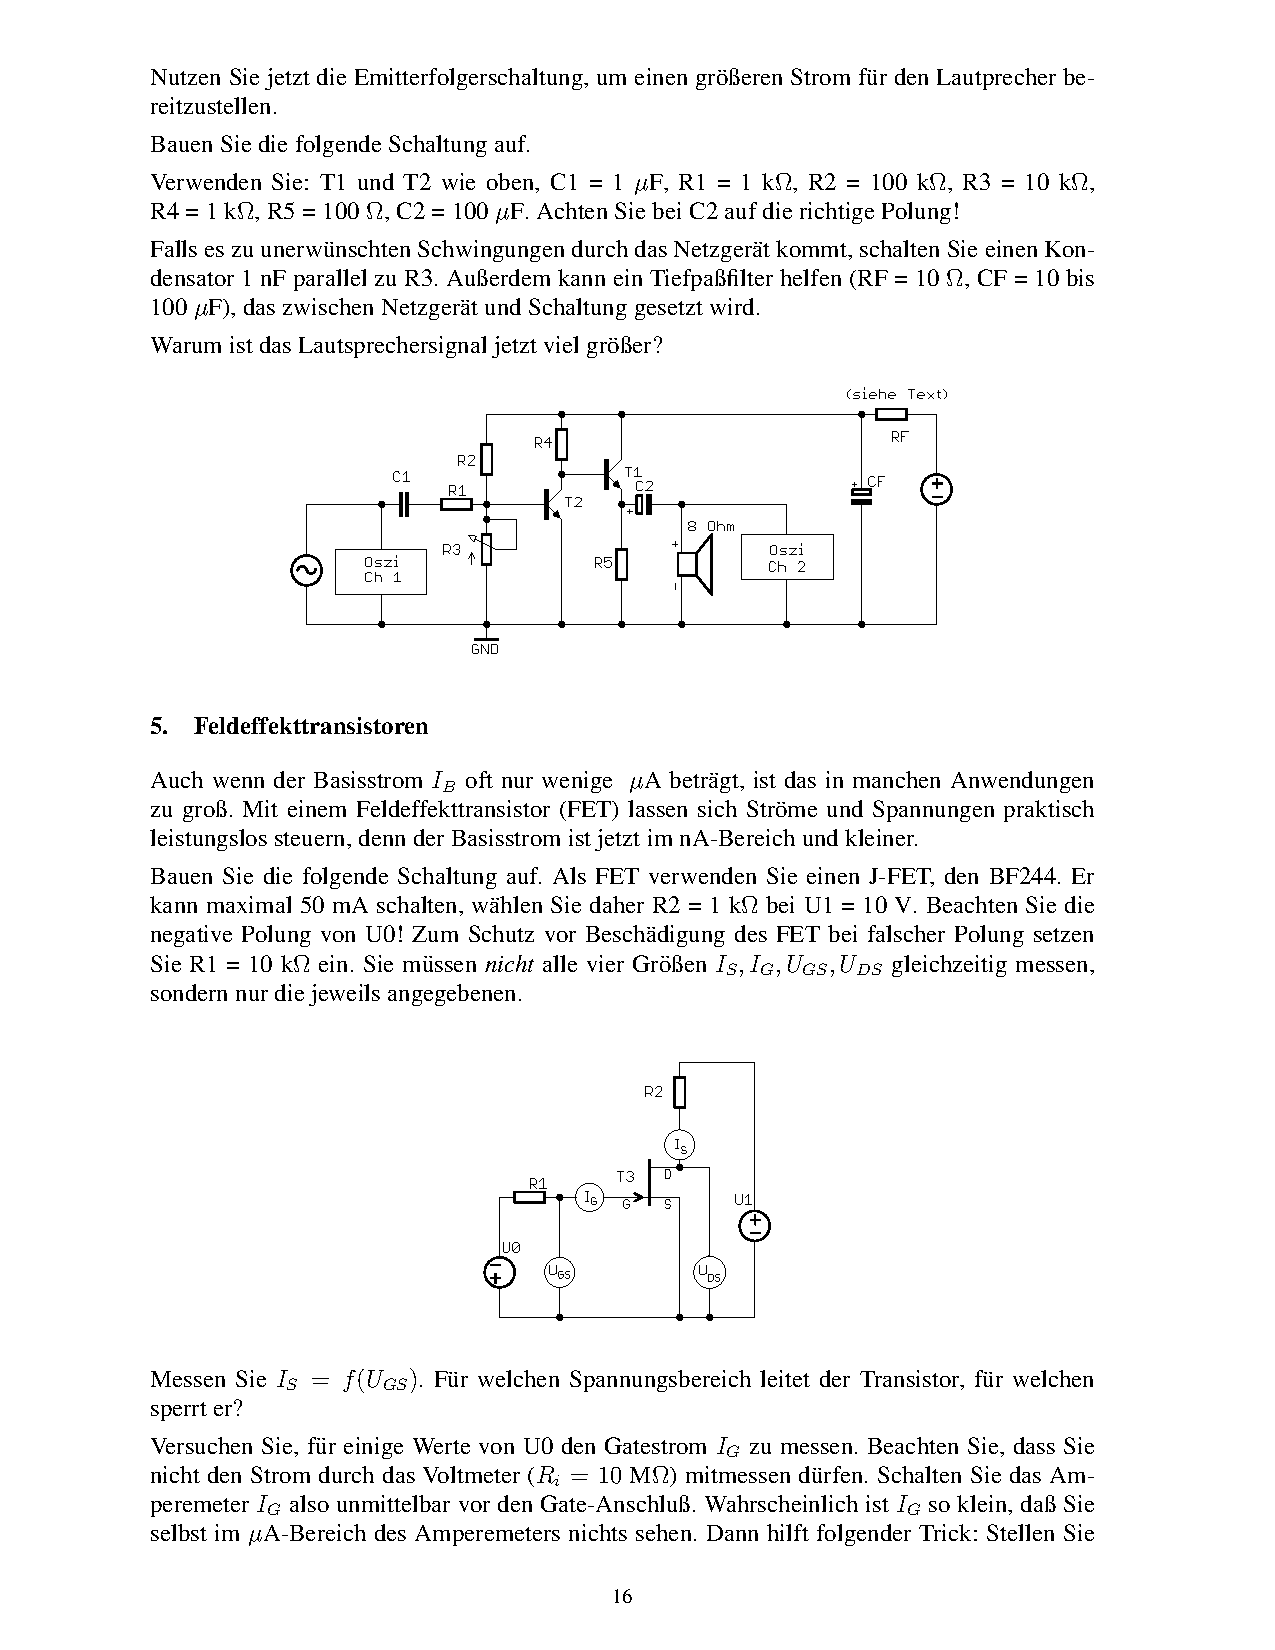
\includegraphics[trim = 10mm 165mm 10mm 69mm, clip, scale = 1]{ep3_14[Page16].pdf}
  	\caption[Schaltskizze für die Messung des Stromverstärkungsfaktors mit zwei hinter einander geschalteten Transistoren und Audioausgabe des verstärkten Signals]{Schaltskizze für die Messung des Stromverstärkungsfaktors mit zwei hinter einander geschalteten Transistoren und Audioausgabe des verstärkten Signals\footnotemark}
  \label{fig:6}
\end{figure}
\footnotetext{Abbildung entnommen von http://www.atlas.uni-wuppertal.de/$\sim$kind/ep3\_14.pdf Seite 16 am 10.11.2014}

\subsection{Versuchsdurchführung}
%erklären, !was! wir machen, !warum! wir das machen und mit welchem ziel
%(wichtig) präzize erklären, wie bei dem versuch vorgegangen und was gemacht wurde
Zur Stromverstärkung wird die Schaltung des sogenannten Emittierfolgers aufgebaut. Es soll $U_a = f(U_e)$ und $I_R = f(I_B)$ bestimmt werden. Als Verstärkungsfaktor wird, da $I_B \ll I_C$ ist, ebenfalls $\beta$ erwartet.
\subsection{Messergebnisse}
%die messwerte in !übersichtlichen! tabellen angegeben
%zu viele kleine tabellen in große tabellen überführen!
%zu große tabellen mit dem [scale]-befehl scalieren oder (falls zu lang) in zwei kleinere tabellen aufteilen
%(wichtig) vor !jeder! tabelle sagen, was gemessen wurde und wie die fehler gewählt wurden und ausreichend !erklären!, !warum! wir unsere fehler grade so gewählt haben
\subsection{Auswertung}
%zuerst !alle! errechneten werte entweder in ganzen sätzen aufzählen, oder in tabellen (übersichtlicher) dargestellen, sowie auf die verwendeten formeln verweisen (die referenzierung der formel kann in der überschrift stehen)
%kurz erwähnen (vor der tabelle), warum wir das ganze ausrechnen bzw. was wir dort ausrechnen
%danach histogramme und plots erstellen, wobei wenn möglich funktionen durch die plots gelegt werden (zur not können auch splines benutzt werden, was aber angegeben werden muss)
%bei fits immer die funktion und das reduzierte chiquadrat mit angegeben, wobei auf verständlichkeit beim entziffern der zehnerpotenzen geachtet werden muss z.b. f(x)=(wert+-fehler)\cdot10^{irgendeine zahl}\cdot x + (wert+-fehler)\cdot10^{irgendeine zahl}
%bei jedem fit erklären, nach welchem zusammenhang gefittet wurde und warum!
%bei plots darauf achten, dass die achsenbeschriftung (auch die tics) die richtige größe haben und die legende im plot nicht die messwerte verdeckt
%kurz die aufgabenstellung abgehandeln
%2-----------------------------------------------2
\subsection{Diskussion}
%(immer) die gemessenen werte und die bestimmten werte über die messfehler mit literaturwerten oder untereinander vergleichen
%in welchem fehlerintervall des messwertes liegt der literaturwert oder der vergleichswert?
%wie ist der relative anteil des fehlers am messwert und damit die qualität unserer messung?
%in einem satz erklären, wie gut unser fehler und damit unsere messung ist
%kurz erläutern, wie systematische fehler unsere messung beeinflusst haben könnten
%(wichtig) zum schluss ansprechen, in wie weit die ergebnisse mit der theoretischen vorhersage übereinstimmen
%--------------------------------------------------------------------------------------------
%falls tabellen mit den messwerten zu lang werden, kann die section mit den messwerten auch hinter der diskussion angefügt bzw. eine section mit dem anhang eingefügt werden.
%1-----------------------------------------------1
\section{Feldeffekttransistoren (FET)}
%kurz das ziel dieses versuchsteiles ansprechen, damit keine zwei überschriften direkt übereinander stehen!
%bei schwierigeren versuchen kann auch der theoretische hintergrund erläutert werden. (mit formeln, herleitungen und erklärungen)
Mit dem Feldeffekttransistor können Ströme und Spannungen fast leistungslos gesteuert werden. (Der Basisstrom beträgt nur wenige Nanoampere)
\subsection{Verwendete Geräte}
%(immer) eine skizze oder ein foto einfügen, die geräte/materialien !nummerieren! und z.b. eine legende dazu schreiben, besser wäre es das ganze in einem Fließtext gut zu beschreiben.
%falls am anfang des versuches nicht klar ist, was alles verwendet wird, wenn möglich erst am ende ein großes foto von den verwendeten materialien machen!\\

\subsection{Verwendete Formeln}
%eine legende kann angefertigt werden, die selbstverständlichen buchstaben müssen nicht extra erklärt werden
%mit knappen erklärungen die !verwendeten! formeln, sowie die zugehörige fehlerrechnung einfügen
%2-----------------------------------------------2
%ab hier kann nochmal in einzelne versuchsteile unterteilt werden
\subsection{Versuchsaufbau}
%skizze zum versuchsaufbau (oder foto) einfügen,   es muss erklärt werden wie das ganze funktioniert und welche speziellen einstellungen verwendet wurden (z.b. welche knöpfe an den geräten für die messung verdreht wurden)

\begin{itemize}
\item	J-FET BF224

\item	R1 10k$\Omega$

\item	R2 1k$\Omega$

\item	U1 10V
\end{itemize}

\begin{figure}[H] 
  \centering
    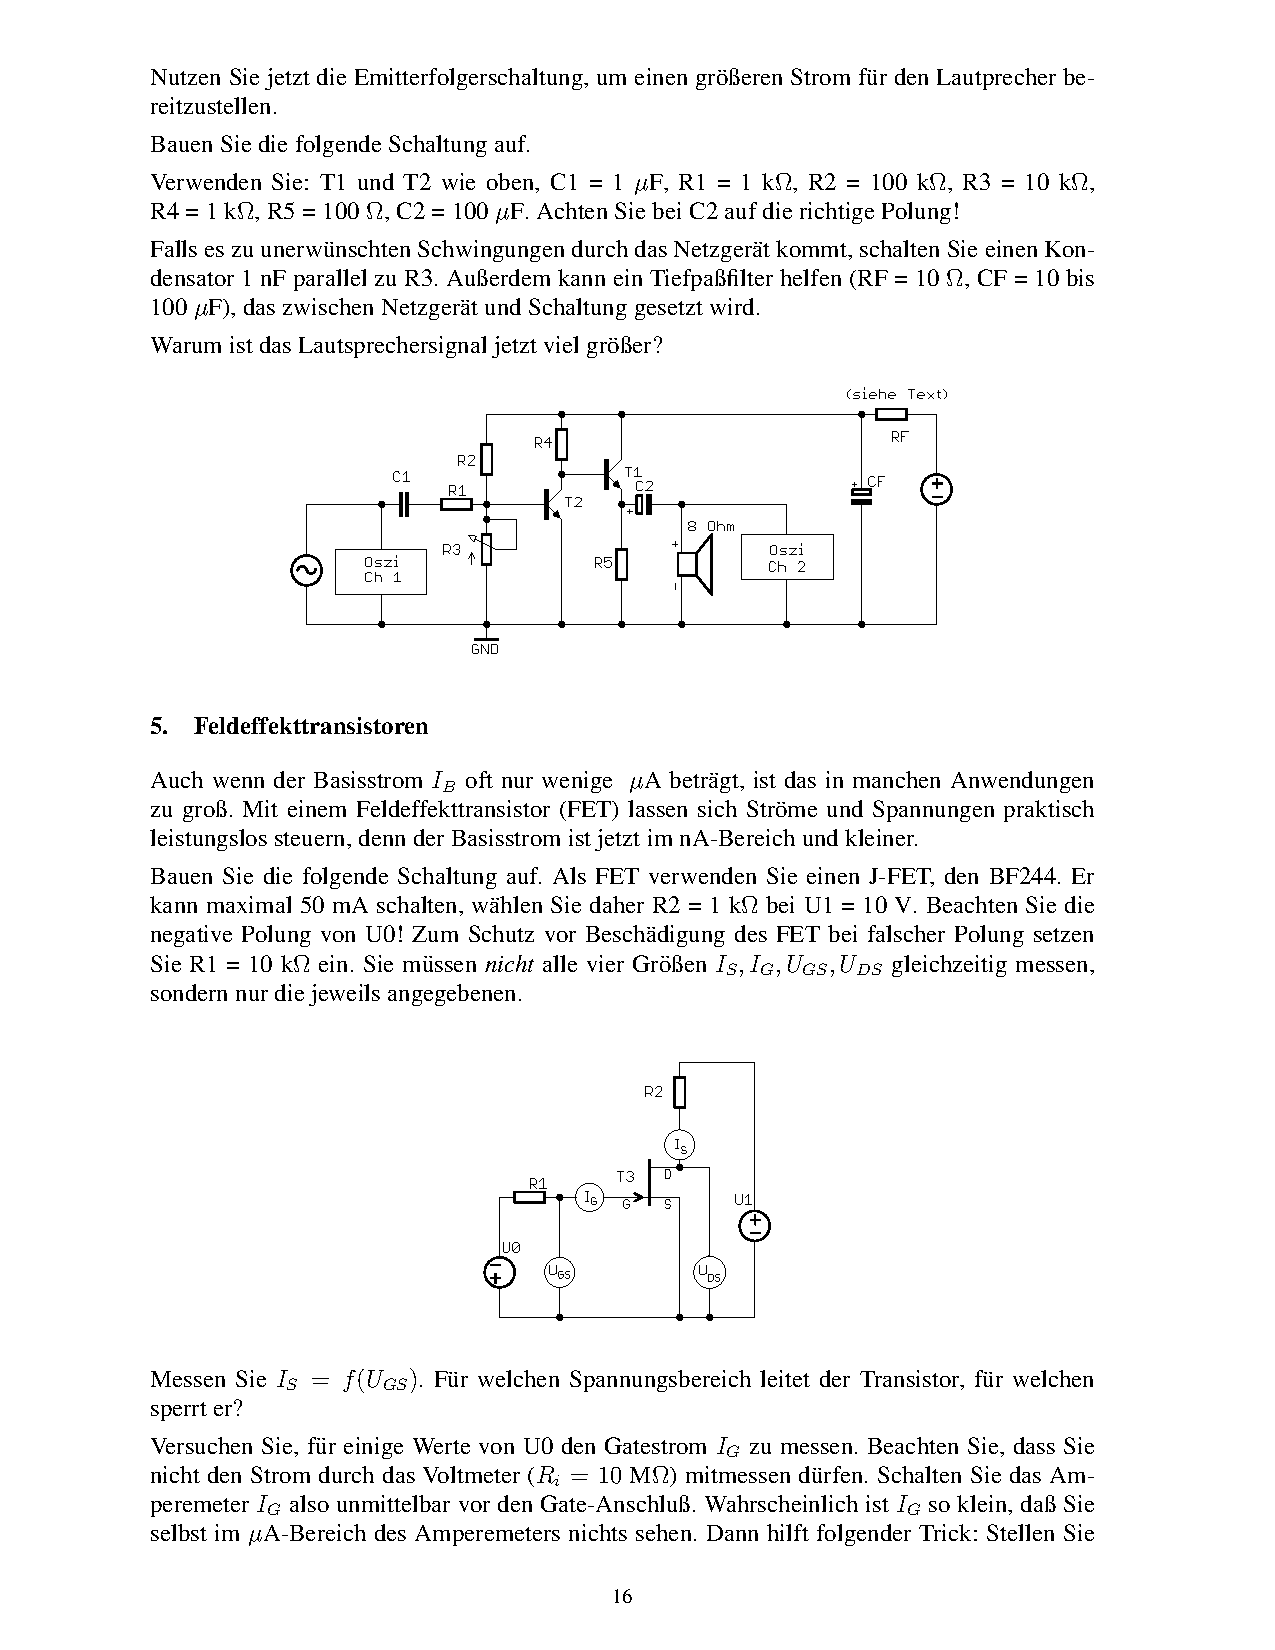
\includegraphics[trim = 10mm 50mm 10mm 174mm, clip, scale = 1]{ep3_14[Page16].pdf}
  	\caption[Schaltskizze für die Messung des Spannungsbereichs, in dem ein Feldaffekttransistor Leitet bzw. nicht]{Schaltskizze für die Messung des Spannungsbereichs, in dem ein Feldaffekttransistor Leitet bzw. nicht\footnotemark}
  \label{fig:7}
\end{figure}
\footnotetext{Abbildung entnommen von http://www.atlas.uni-wuppertal.de/$\sim$kind/ep3\_14.pdf Seite 16 am 10.11.2014}

\subsection{Versuchsdurchführung}
%erklären, !was! wir machen, !warum! wir das machen und mit welchem ziel
%(wichtig) präzize erklären, wie bei dem versuch vorgegangen und was gemacht wurde
Der Feldeffekttransistor kann über die Gatespannung $U_{GS}$ mit nur wenigen \unit{nA} angesteuert werden, sodass ein Feld entsteht, welches den Stromfluss $I_S$ reguliert. Dafür wird $I_S = f(U_{GS})$ ermittelt.
\subsection{Messergebnisse}
%die messwerte in !übersichtlichen! tabellen angegeben
%zu viele kleine tabellen in große tabellen überführen!
%zu große tabellen mit dem [scale]-befehl scalieren oder (falls zu lang) in zwei kleinere tabellen aufteilen
%(wichtig) vor !jeder! tabelle sagen, was gemessen wurde und wie die fehler gewählt wurden und ausreichend !erklären!, !warum! wir unsere fehler grade so gewählt haben
\subsection{Auswertung}
%zuerst !alle! errechneten werte entweder in ganzen sätzen aufzählen, oder in tabellen (übersichtlicher) dargestellen, sowie auf die verwendeten formeln verweisen (die referenzierung der formel kann in der überschrift stehen)
%kurz erwähnen (vor der tabelle), warum wir das ganze ausrechnen bzw. was wir dort ausrechnen
%danach histogramme und plots erstellen, wobei wenn möglich funktionen durch die plots gelegt werden (zur not können auch splines benutzt werden, was aber angegeben werden muss)
%bei fits immer die funktion und das reduzierte chiquadrat mit angegeben, wobei auf verständlichkeit beim entziffern der zehnerpotenzen geachtet werden muss z.b. f(x)=(wert+-fehler)\cdot10^{irgendeine zahl}\cdot x + (wert+-fehler)\cdot10^{irgendeine zahl}
%bei jedem fit erklären, nach welchem zusammenhang gefittet wurde und warum!
%bei plots darauf achten, dass die achsenbeschriftung (auch die tics) die richtige größe haben und die legende im plot nicht die messwerte verdeckt
%kurz die aufgabenstellung abgehandeln
%2-----------------------------------------------2
\subsection{Diskussion}
%(immer) die gemessenen werte und die bestimmten werte über die messfehler mit literaturwerten oder untereinander vergleichen
%in welchem fehlerintervall des messwertes liegt der literaturwert oder der vergleichswert?
%wie ist der relative anteil des fehlers am messwert und damit die qualität unserer messung?
%in einem satz erklären, wie gut unser fehler und damit unsere messung ist
%kurz erläutern, wie systematische fehler unsere messung beeinflusst haben könnten
%(wichtig) zum schluss ansprechen, in wie weit die ergebnisse mit der theoretischen vorhersage übereinstimmen
%--------------------------------------------------------------------------------------------
%falls tabellen mit den messwerten zu lang werden, kann die section mit den messwerten auch hinter der diskussion angefügt bzw. eine section mit dem anhang eingefügt werden.
%1-----------------------------------------------1
\section{Spannungsstabilisierung mit Transistoren}
%kurz das ziel dieses versuchsteiles ansprechen, damit keine zwei überschriften direkt übereinander stehen!
%bei schwierigeren versuchen kann auch der theoretische hintergrund erläutert werden. (mit formeln, herleitungen und erklärungen)
Analog zum letzten Versuch kann mit einer Zenerdiode eine konstante Gleichspannung erzeugt werden. Aufgrund des Vorwiderstandes war es aber nicht möglich hohe Ausgangsströme zu erreichen. Führt man die Zehnerspannung über einen Emittierfolger (Stromverstärker), so sind wesentlich höhere Ströme möglich.
\subsection{Verwendete Geräte}
%(immer) eine skizze oder ein foto einfügen, die geräte/materialien !nummerieren! und z.b. eine legende dazu schreiben, besser wäre es das ganze in einem Fließtext gut zu beschreiben.
%falls am anfang des versuches nicht klar ist, was alles verwendet wird, wenn möglich erst am ende ein großes foto von den verwendeten materialien machen!\\
\subsection{Verwendete Formeln}
%eine legende kann angefertigt werden, die selbstverständlichen buchstaben müssen nicht extra erklärt werden
%mit knappen erklärungen die !verwendeten! formeln, sowie die zugehörige fehlerrechnung einfügen
%2-----------------------------------------------2
%ab hier kann nochmal in einzelne versuchsteile unterteilt werden
\subsection{Versuchsaufbau}
%skizze zum versuchsaufbau (oder foto) einfügen,   es muss erklärt werden wie das ganze funktioniert und welche speziellen einstellungen verwendet wurden (z.b. welche knöpfe an den geräten für die messung verdreht wurden)

\begin{itemize}
\item	D1 Zenerdiode

\item	T1 BD137

\item	R1 200$\Omega$

\item	R2 470$\Omega$ Potentiometer

\item	R3 = 20$\Omega$

\item	100nF
\end{itemize}

\begin{figure}[H] 
  \centering
    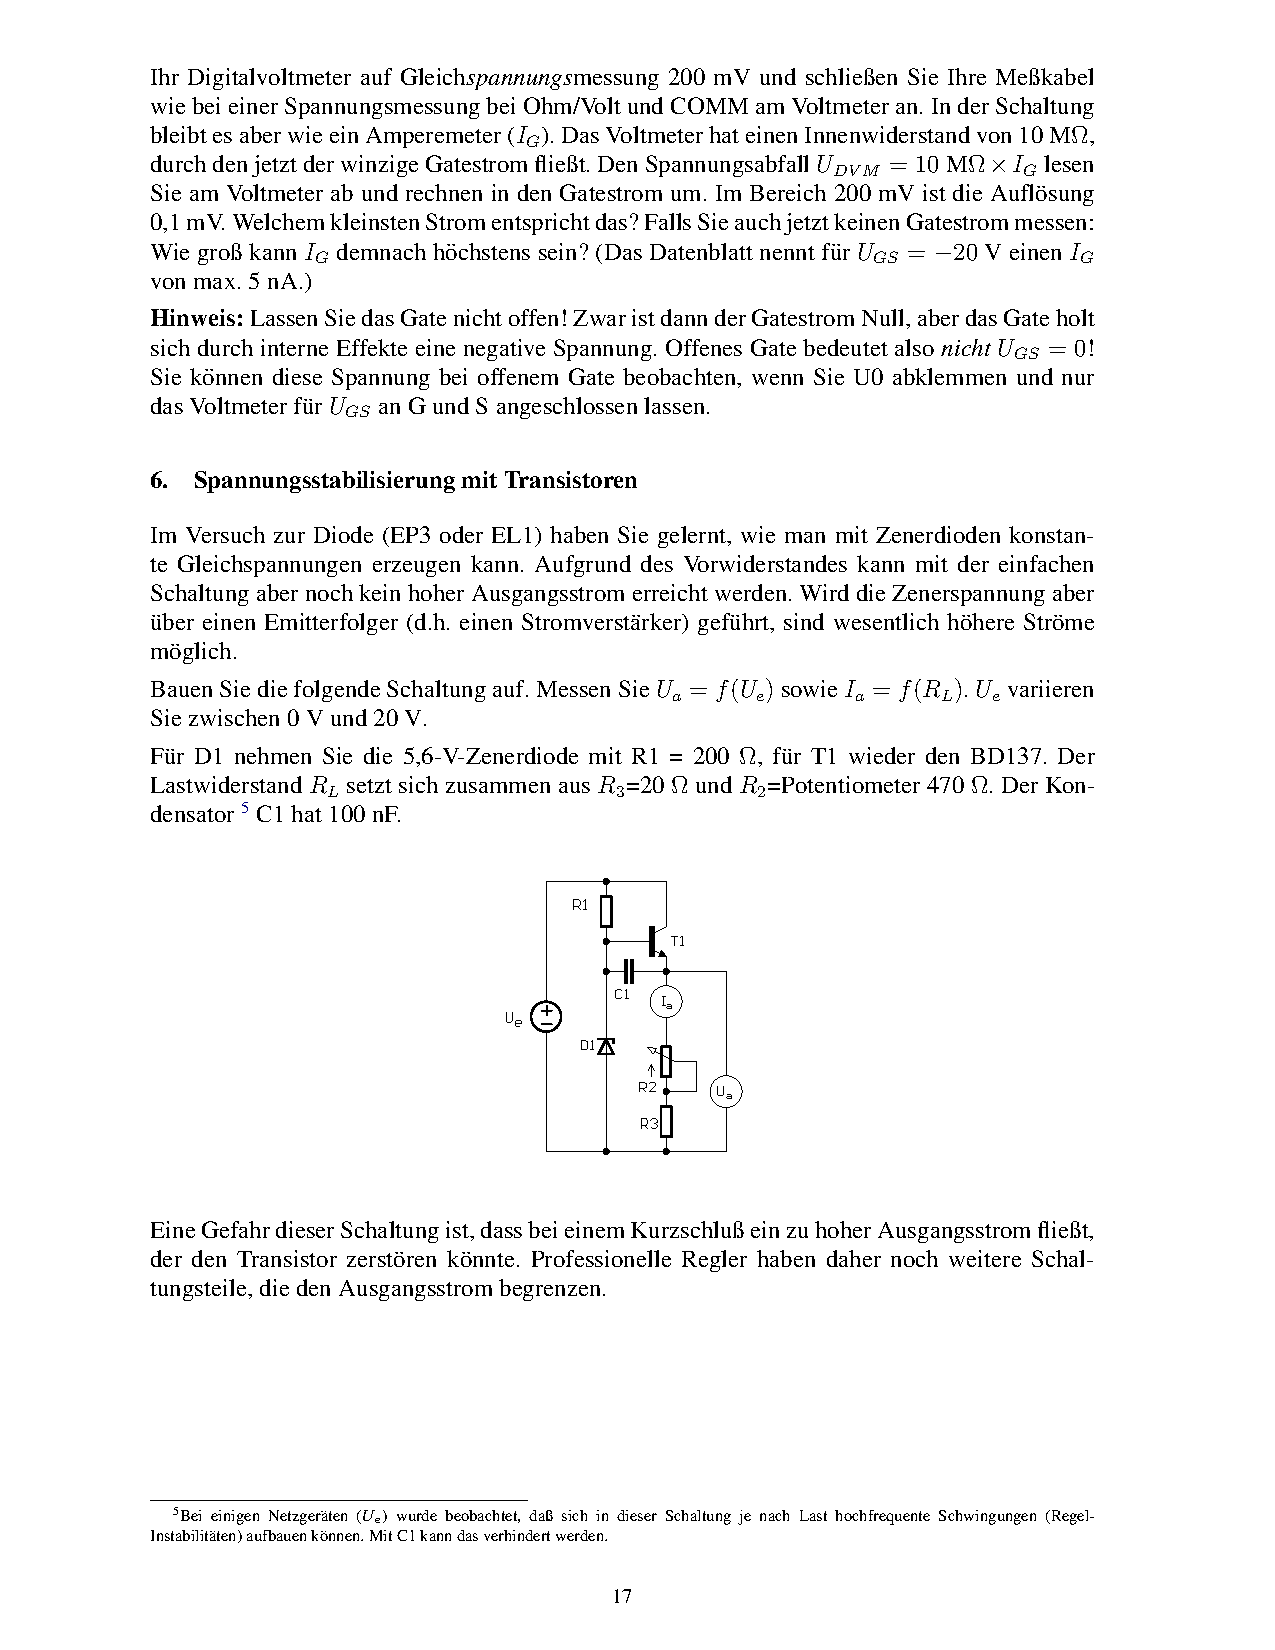
\includegraphics[trim = 10mm 80mm 10mm 140mm, clip, scale = 1]{ep3_14[Page17].pdf}
  	\caption[Schaltskizze für die Messung der Spannungsstabilisierung durch Transistoren]{Schaltskizze für die Messung der Spannungsstabilisierung durch Transistoren\footnotemark}
  \label{fig:8}
\end{figure}
\footnotetext{Abbildung entnommen von http://www.atlas.uni-wuppertal.de/$\sim$kind/ep3\_14.pdf Seite 16 am 10.11.2014}

\subsection{Versuchsdurchführung}
%erklären, !was! wir machen, !warum! wir das machen und mit welchem ziel
%(wichtig) präzize erklären, wie bei dem versuch vorgegangen und was gemacht wurde

\subsection{Messergebnisse}
%die messwerte in !übersichtlichen! tabellen angegeben
%zu viele kleine tabellen in große tabellen überführen!
%zu große tabellen mit dem [scale]-befehl scalieren oder (falls zu lang) in zwei kleinere tabellen aufteilen
%(wichtig) vor !jeder! tabelle sagen, was gemessen wurde und wie die fehler gewählt wurden und ausreichend !erklären!, !warum! wir unsere fehler grade so gewählt haben
\subsection{Auswertung}
%zuerst !alle! errechneten werte entweder in ganzen sätzen aufzählen, oder in tabellen (übersichtlicher) dargestellen, sowie auf die verwendeten formeln verweisen (die referenzierung der formel kann in der überschrift stehen)
%kurz erwähnen (vor der tabelle), warum wir das ganze ausrechnen bzw. was wir dort ausrechnen
%danach histogramme und plots erstellen, wobei wenn möglich funktionen durch die plots gelegt werden (zur not können auch splines benutzt werden, was aber angegeben werden muss)
%bei fits immer die funktion und das reduzierte chiquadrat mit angegeben, wobei auf verständlichkeit beim entziffern der zehnerpotenzen geachtet werden muss z.b. f(x)=(wert+-fehler)\cdot10^{irgendeine zahl}\cdot x + (wert+-fehler)\cdot10^{irgendeine zahl}
%bei jedem fit erklären, nach welchem zusammenhang gefittet wurde und warum!
%bei plots darauf achten, dass die achsenbeschriftung (auch die tics) die richtige größe haben und die legende im plot nicht die messwerte verdeckt
%kurz die aufgabenstellung abgehandeln
%2-----------------------------------------------2
\subsection{Diskussion}
%(immer) die gemessenen werte und die bestimmten werte über die messfehler mit literaturwerten oder untereinander vergleichen
%in welchem fehlerintervall des messwertes liegt der literaturwert oder der vergleichswert?
%wie ist der relative anteil des fehlers am messwert und damit die qualität unserer messung?
%in einem satz erklären, wie gut unser fehler und damit unsere messung ist
%kurz erläutern, wie systematische fehler unsere messung beeinflusst haben könnten
%(wichtig) zum schluss ansprechen, in wie weit die ergebnisse mit der theoretischen vorhersage übereinstimmen
%--------------------------------------------------------------------------------------------
%falls tabellen mit den messwerten zu lang werden, kann die section mit den messwerten auch hinter der diskussion angefügt bzw. eine section mit dem anhang eingefügt werden.
%1-----------------------------------------------1

\section{Fazit}
%im fazit nochmal alles zusammenfassen und den verlauf der messung abschätzen
%gravierende sytematische probleme bei den messungen nochmal betonen und die wertigkeit unserer ergebnisse einordnen
\end{document}

